\documentclass{beamer}

%\useoutertheme[glossy]{wuerzburg}
\useinnertheme[shadow,outline]{chamfered}
%\usecolortheme{shark}
\usecolortheme{beaver}
\beamertemplatenavigationsymbolsempty

\usefonttheme{professionalfonts}
\let\digamma\relax
\usepackage[scale=0.85,stdmathitalics=true,romanfamily=casual]{lucimatx}
\usefonttheme[stillsansseriftext]{serif}



\usepackage{fancyvrb}

%% Fancy syntax coloring via pygments
\usepackage{minted}
\definecolor{bg}{rgb}{0.95,0.95,0.95}
\usemintedstyle{borland}


\newenvironment{Rcode}
{\VerbatimEnvironment
 \begin{minted}[fontsize=\scriptsize,baselinestretch=1]{r}}%
{\end{minted}}

\newenvironment{Pcode}
{\VerbatimEnvironment
 \begin{minted}[fontsize=\scriptsize,baselinestretch=1]{python}}%
{\end{minted}}

\newenvironment{Code}[1]
{\VerbatimEnvironment
 \begin{minted}[fontsize=\scriptsize,baselinestretch=1]{#1}}%
{\end{minted}}


\usepackage{textfit} % commands \scaletoheight{height}{text} and \scaletowidth{width}{text}

\usepackage{tikz}

\usepackage{tcolorbox}

\newtheorem{Alert}{Alert}
\newtheorem{Highlight}{Highlight}

\newcommand{\Species}[1]{{\rmfamily \itshape #1}}
\newcommand{\Real}{\ensuremath{\mathbb{R}}}
\newcommand{\RealN}{\ensuremath{\mathbb{R}^n}}
\newcommand{\RealP}{\ensuremath{\mathbb{R}^p}}
\newcommand{\Mtx}[1]{\ensuremath{\mathbf{#1}}}
\newcommand{\Inv}[1]{\ensuremath{#1^{-1}}}
\newcommand{\InvMtx}[1]{\ensuremath{\mathbf{#1}^{-1}}}
\newcommand{\Red}[1]{\textcolor{red}{#1}}
\newcommand{\PsInv}[1]{\ensuremath{\mathbf{#1}^{+}}}

\usepackage{booktabs}



% --- Macro \xvec
% From a tex.stackexchange.com answer by Todd Lehman
% http://tex.stackexchange.com/questions/44017/dot-notation-for-derivative-of-a-vector
\makeatletter
\newlength\xvec@height%
\newlength\xvec@depth%
\newlength\xvec@width%
\newcommand{\xvec}[2][]{%
  \ifmmode%
    \settoheight{\xvec@height}{$#2$}%
    \settodepth{\xvec@depth}{$#2$}%
    \settowidth{\xvec@width}{$#2$}%
  \else%
    \settoheight{\xvec@height}{#2}%
    \settodepth{\xvec@depth}{#2}%
    \settowidth{\xvec@width}{#2}%
  \fi%
  \def\xvec@arg{#1}%
  \def\xvec@dd{:}%
  \def\xvec@d{.}%
  \raisebox{.2ex}{\raisebox{\xvec@height}{\rlap{%
    \kern.05em%  (Because left edge of drawing is at .05em)
    \begin{tikzpicture}[scale=1]
    \pgfsetroundcap
    \draw (.05em,0)--(\xvec@width-.05em,0);
    \draw (\xvec@width-.05em,0)--(\xvec@width-.15em, .075em);
    \draw (\xvec@width-.05em,0)--(\xvec@width-.15em,-.075em);
    \ifx\xvec@arg\xvec@d%
      \fill(\xvec@width*.45,.5ex) circle (.5pt);%
    \else\ifx\xvec@arg\xvec@dd%
      \fill(\xvec@width*.30,.5ex) circle (.5pt);%
      \fill(\xvec@width*.65,.5ex) circle (.5pt);%
    \fi\fi%
    \end{tikzpicture}%
  }}}%
  #2%
}
\makeatother

% --- Override \vec with an invocation of \xvec.
\let\stdvec\vec
\renewcommand{\vec}[1]{\xvec[]{#1}}
% --- Define \dvec and \ddvec for dotted and double-dotted vectors.
\newcommand{\dvec}[1]{\xvec[.]{#1}}
\newcommand{\ddvec}[1]{\xvec[:]{#1}}


\usepackage{pifont}
\newcommand{\weblink}{\ding{43}}  % hand with pointing finger

\definecolor{links}{HTML}{2A1B81}
\hypersetup{colorlinks,linkcolor=,urlcolor=magenta}

\usepackage{pdfpages}

\parskip=0.5em

%===========================================================
% Title Info
\title{Scientific Computing for Biologists}
\subtitle{Lecture 11: Resampling methods and other non-parametric appraoches} % (optional)

\author{Instructor: Paul M. Magwene}
\date{13 November 2012}


\begin{document}

\begin{frame}
\titlepage
\end{frame}



\begin{frame}
  \frametitle{Goals of Resampling Methods}

\begin{block}{Goal}
We have estimated some statistic of interest, $S$, for a set of observed data. We want to know whether the value of $S$ we estimate, $\widehat{s}$, is likely to have been generated by chance or under a model captured by an appropriate null hypothesis.
\end{block}


\begin{block}{Approach}
Randomization tests and related methods allow one to address these questions for many types of statistics that are not amenable to classical analysis.
\end{block}



\end{frame}
%@nonl
%@-node:pmagwene.20061106201501:Goals
%@+node:pmagwene.20061128102139:Advantages


\begin{frame}
  \frametitle{Advantages of Resampling Methods}


In general, resampling methods are:
\begin{itemize}
    \item Computer intensive 
    \item Require few assumptions about the distributional properties 
    \item Robust
\end{itemize}

\end{frame}
%@nonl
%@-node:pmagwene.20061128102139:Advantages
%@+node:pmagwene.20061127233248:Randomization tests
%@+node:pmagwene.20061127234838:overview

\begin{frame}
  \frametitle{Overview of Randomization Tests}

\begin{block}{Basic Idea}
Compare $\widehat{s}$ to the distribution of estimates of $S$ obtained by randomly reordering the data.
\end{block}

\end{frame}
%@nonl
%@-node:pmagwene.20061127234838:overview
%@+node:pmagwene.20061127235344.1:example

\begin{frame}
  \frametitle{Randomization tests: Example}

Consider the following measurements of mandible length (in mm) from skeletons of male and female golden jackals (\emph{Canis aureus}).

\begin{itemize}
    \item Male: 120, 107, 110, 116, 114, 11, 113, 117, 114, 112
    \item Female: 110, 111, 107, 108, 110, 105, 107, 106, 111, 111
\end{itemize}

\begin{block}{Question}
Are the mean values for the two sexes different?
\end{block}

\end{frame}
%@nonl
%@-node:pmagwene.20061127235344.1:example
%@+node:pmagwene.20061128135753:example II
\begin{frame}
  \frametitle{Randomization tests: Example cont}

The means for the two sexes are: 
\begin{itemize}
    \item $\bar{x}_{male} = 113.4$
    \item $\bar{x}_{female} = 108.6$ 
\end{itemize}

Standard deviations:
\begin{itemize}
    \item $s_{male} = 3.72$ 
    \item $s_{female} = 2.27$.
\end{itemize}
\medskip

To construct the randomization test:
\begin{itemize}
    \item generate a large number of samples where we randomly reallocate 10 of the specimens to the male group and the remaining 10 we designate as female. 
    \item for each randomized sample calculate the difference in means between the male and female groups
    \item Examine the distribution of the randomization distribution and ask whether the observed difference in means is atypical.

\end{itemize}




\end{frame}
%@nonl
%@-node:pmagwene.20061128135753:example II
%@+node:pmagwene.20061128141008:example III
\begin{frame}
  \frametitle{Randomization tests: Example cont}


\begin{center}
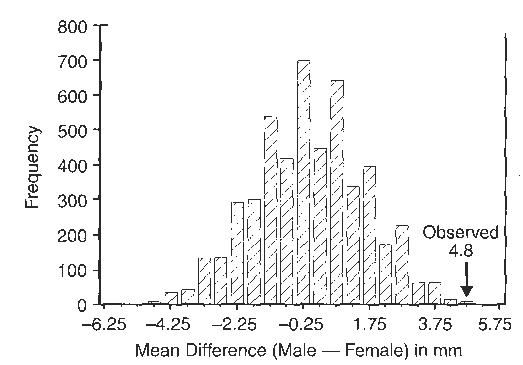
\includegraphics[height=2.5in]{jackal-distn2}
\end{center}



\end{frame}
%@nonl
%@-node:pmagwene.20061128141008:example III
%@+node:pmagwene.20061127235344:advantages and limitations

\begin{frame}
  \frametitle{Advantages and Limitations of Randomization Tests}

Advantages:
\begin{itemize}
    \item Valid even without a random sample
    \item Can be designed to take particulars of a particular statistic into account
    \item When there is a classical, parametric equivalent there is often good agreement
\end{itemize}

Limitations:
\begin{itemize}
    \item Not possible to generalize to a population of interest
%    \item Generally limited to hypotheses involving two or more groups
\end{itemize}

\end{frame}
%@nonl
%@-node:pmagwene.20061127235344:advantages and limitations
%@-node:pmagwene.20061127233248:Randomization tests
%@+node:pmagwene.20061127233327.2:Monte Carlo Methods
%@+node:pmagwene.20061128000033.6:overview
%@-node:pmagwene.20061128000033.6:overview
%@+node:pmagwene.20061128000033.7:advantages and limitations
%@-node:pmagwene.20061128000033.7:advantages and limitations
%@+node:pmagwene.20061128000033.8:examples
%@-node:pmagwene.20061128000033.8:examples
%@-node:pmagwene.20061127233327.2:Monte Carlo Methods
%@+node:pmagwene.20061127233327:Jackknife
%@+node:pmagwene.20061128000033:overview

\begin{frame}
  \frametitle{Overiew of Jackknife Methodology}

\begin{block}{Basic Idea}
Turn the problem of estimating any parameter of interest for $n$ observations into a problem of estimating a sample mean.
\end{block}

\begin{block}{Basic Mechanics}
Calculate pseudovalues of $S$, $s^*$, leaving out a single observation at a time. Calculate mean and standard errors of pseudovalues to estimate confidence intervals for $\widehat{s}$.

\end{block}




\end{frame}
%@nonl
%@-node:pmagwene.20061128000033:overview
%@+node:pmagwene.20061128100749:motivation

\begin{frame}
  \frametitle{Motivation for Jackknifing}

\begin{itemize}
    \item Let $\bar{x} = 1/n \sum_{i=1}^{n}x_i$ denote the mean for a sample of size $n$.

    \item Let 
\[
\bar{x}_{-j} = \frac{1}{n-1} \sum_{i \neq 1}^{n}x_i
\]
denote the sample mean with the $j$th observation removed.

    \item If we know both $\bar{x}$ and $\bar{x}_{-j}$ we can compute the value of the $j$th point as
\[
x_j = n\bar{x} - (n-1)\bar{x}_{-j}
\]


\end{itemize}

\end{frame}
%@nonl
%@-node:pmagwene.20061128100749:motivation
%@+node:pmagwene.20061128103843:motivation II

\begin{frame}
  \frametitle{Motivation for Jackknifing II}

\begin{itemize}
    \item Now assume we're interested in some arbitrarily complex statistic that is a function of the $n$ data points:
\[
\widehat{\Theta} = \phi(x_1, x_2, \cdots, x_{i-1}, x_i, x_{i+1}, \cdots x_n)
\]

    \item We define the $j$th \textbf{partial estimate} of $\Theta$ as
\[
\widehat{\Theta}_j = \phi(x_1, x_2, \cdots, x_{i-1}, x_{i+1}, \cdots x_n)
\]

    \item By analogy with the previous formula we define the $j$th \textbf{pseudovalue} as:
\[
\widehat{\Theta^*}_j = n \widehat{\Theta} - (n-1)\widehat{\Theta}_j 
\]



\end{itemize}

\end{frame}
%@nonl
%@-node:pmagwene.20061128103843:motivation II
%@+node:pmagwene.20061128104108:motivation III
\begin{frame}
  \frametitle{Motivation for Jackknifing III}

\begin{itemize}
    \item From the pseudovalues we can calculate a \textbf{jackknife estimate} of $\Theta$ as follows
\[
\widehat{\Theta^*} = \frac{1}{n} \sum_{i=1}{n}\widehat{\Theta^*}_i
\]

    \item We can approximate the standard error of $\widehat{\Theta^*}$ by calculating the standard error
\[
SE_{jack} = \sqrt{\frac{Var(\widehat{\Theta^*}_j)}{n}}
\]


    \item An approximate $(1-\alpha)$\% confidence interval is given by
\[
\widehat{\Theta^*} \pm t_{\alpha/2, n-1} SE_{jack}
\]

where $t_{\alpha/2, n-1}$ is the valued that is exceeded with probability $\alpha/2$ for the t-distribution with n-1 degrees of freedom.

\end{itemize}

\end{frame}
%@nonl
%@-node:pmagwene.20061128104108:motivation III
%@+node:pmagwene.20061128000033.2:examples

\begin{frame}
  \frametitle{Jackknife Estimates: Example}

Suppose we have a random sample of size $n=20$ that consists of the following observations: 3.56, 0.69, 0.10, 1.84, 3.93, 1.25, 0.18, 1.13, 0.27, 0.50, 0.01, 0.61, 0.82, 1.70, 0.39, 0.11, 1.20, 1.21, 0.72
\medskip

Let's use the jackknife to estimate confidence intervals for the standard deviation, $\sigma$ of this sample.

\begin{itemize}
    \item We calculate the jackknife pseudovalues, $\widehat{\sigma^*_1}, \ldots, \widehat{\sigma^*_20}$
    \item The mean of the jackknife pseudovalues, $\widehat{\sigma^*} = 1.096$.
    \item The variance of the pseudovalues, $Var(\widehat{\Theta^*}_j) = 1.488$
    \item The standard error of the pseudovalues, $\sqrt{\frac{Var(\widehat{\Theta^*}_j)}{n}} = 0.273$.
    \item The approximate 95\% confidence interval is: $1.096 \pm 2.09 \times 0.273 = (0.53, 1.67)$

\end{itemize}



\end{frame}
%@nonl
%@-node:pmagwene.20061128000033.2:examples
%@+node:pmagwene.20061128000033.1:advantages and limitations

\begin{frame}
  \frametitle{Advantages and Limitations of Jackknife Estimates}

Advantages:
\begin{itemize}
    \item Simple to calculate and not particularly computer intensive
    \item Jackknife estimates reduce bias
\end{itemize}

Limitations:
\begin{itemize}
    \item Works best when observed sample is moderately large
    \item Jackknife confidence intervals can sometimes over or underestimate the true confidence interval so simulation studies to test the robustness of the jackknife for a statistic of interest are often warranted
%    \item Generally limited to hypotheses involving two or more groups
\end{itemize}

\end{frame}
%@nonl
%@-node:pmagwene.20061128000033.1:advantages and limitations
%@-node:pmagwene.20061127233327:Jackknife
%@+node:pmagwene.20061127233327.1:Bootstrap
%@+node:pmagwene.20061128000033.3:overview

\begin{frame}
  \frametitle{Bootstrap: Overview}
  
\begin{block}{Basic Idea}
\begin{itemize}
    \item In the absence of a priori knowledge about a population, the distribution of values in random samples is the best guide to the distribution of values in the population as a whole.

    \item If we are unable to resample the population to learn about the distribution of a statistic, $S$, the best proxy is the resample our original sample. Resampling is done \emph{with replacement} in contrast to randomization tests.
\end{itemize}
\end{block}


\begin{block}{Basic Mechanics}
Generate a large number of \textbf{bootstrap samples} by repeatedly resampling the original set of observations.  Approximate the standard error of $S$ based on the set of bootstrap samples. Estimate bias and/or confidence intervals based on bootstrap samples.

\end{block}

  

\end{frame}
%@nonl
%@-node:pmagwene.20061128000033.3:overview
%@+node:pmagwene.20061128115932:bootstrap CIs: standard limits

\begin{frame}
  \frametitle{Bootstrap: Standard confidence limits}
  
Simple method for obtaining bootstrap confidence limits is to assume that $\widehat{\Theta}$ has an approximately normal distribution and the bootstrap sampling gives a good approximation to the standard deviation of the statistic of interest.
\medskip

Standard Bootstrap Confidence Limits:

\[
\mbox{Estimate} \pm z_{\alpha/2} (\mbox{bootstrap standard deviation})
\]

where 'Estimate' is the estimate of the parameter of interest based on the initial sample and the 'bootstrap standard deviation' is based on the variance of the bootstrap samples.

\end{frame}
%@nonl
%@-node:pmagwene.20061128115932:bootstrap CIs: standard limits
%@+node:pmagwene.20061128115932.1:bootstrap CIs: percentile limits
\begin{frame}
  \frametitle{Bootrap: Percentile confidence limits}
  
Calculate confidence intervals directly from the bootstrap samples themselves.

\begin{itemize}
    \item Makes no assumptions about normality
    \item Requires fairly large bootstrap samples ($\geq 1000$ for 95\% CIs, $\geq 5000$ for 99\% CIs)
\end{itemize}

Efron's percentile confidence limits:
\begin{itemize}
    \item $(\widehat{\Theta}_{L,\alpha/2}, \widehat{\Theta}_{H,\alpha/2})$ where $\widehat{\Theta}_{L,\alpha/2}$ is the estimate of $\Theta$ from the bootstrap distribution such that a fraction $\alpha/2$ of all bootstrap estimates are less than this value, likewise for the upper limit $\widehat{\Theta}_{H,\alpha/2}$
\end{itemize}


\end{frame}
%@nonl
%@-node:pmagwene.20061128115932.1:bootstrap CIs: percentile limits
%@+node:pmagwene.20061128000033.5:examples

\begin{frame}
  \frametitle{Bootstrap: Examples}
  
Consider the same sample used to illustrate the jackknife with observations: 3.56, 0.69, 0.10, 1.84, 3.93, 1.25, 0.18, 1.13, 0.27, 0.50, 0.01, 0.61, 0.82, 1.70, 0.39, 0.11, 1.20, 1.21, 0.72
\medskip

Let's use the bootstrap to estimate the confidence interval for the standard deviation of the distribution this sample is drawn from.
\smallskip

\begin{itemize}
    \item the sample estimate of the standard deviation is, $\widehat{\sigma} = 1.06$
    \item generated 1000 bootstrap samples
    \begin{itemize}
        \item mean of the bootstrap samples = 0.97
        \item standard error of the bootstrap samples = 0.25
    \end{itemize}
    \item Standard 95\% confidence limits: $1.06 \pm 1.96(0.25) = (0.57, 1.55)$
\end{itemize}
        

\end{frame}
%@nonl
%@-node:pmagwene.20061128000033.5:examples
%@+node:pmagwene.20061128000033.4:advantages and limitations

\begin{frame}
  \frametitle{Bootstrap: Advantages and Limitations}

Advantages:
\begin{itemize}
    \item Robust
    \item Can be applied to arbitrary statistics of interest
\end{itemize}

Limitations:
\begin{itemize}
    \item Works best when observed sample is moderately large
    \item Requires a fair amount of computing power (not typically a problem these days)
    \item Variety of complex procedure for estimating confidence intervals, none clearly preferable in all situations
\end{itemize}

\end{frame}

%===========================================================
\begin{frame}
  \frametitle{Bootstrap vs. Jackknife}

\begin{center}
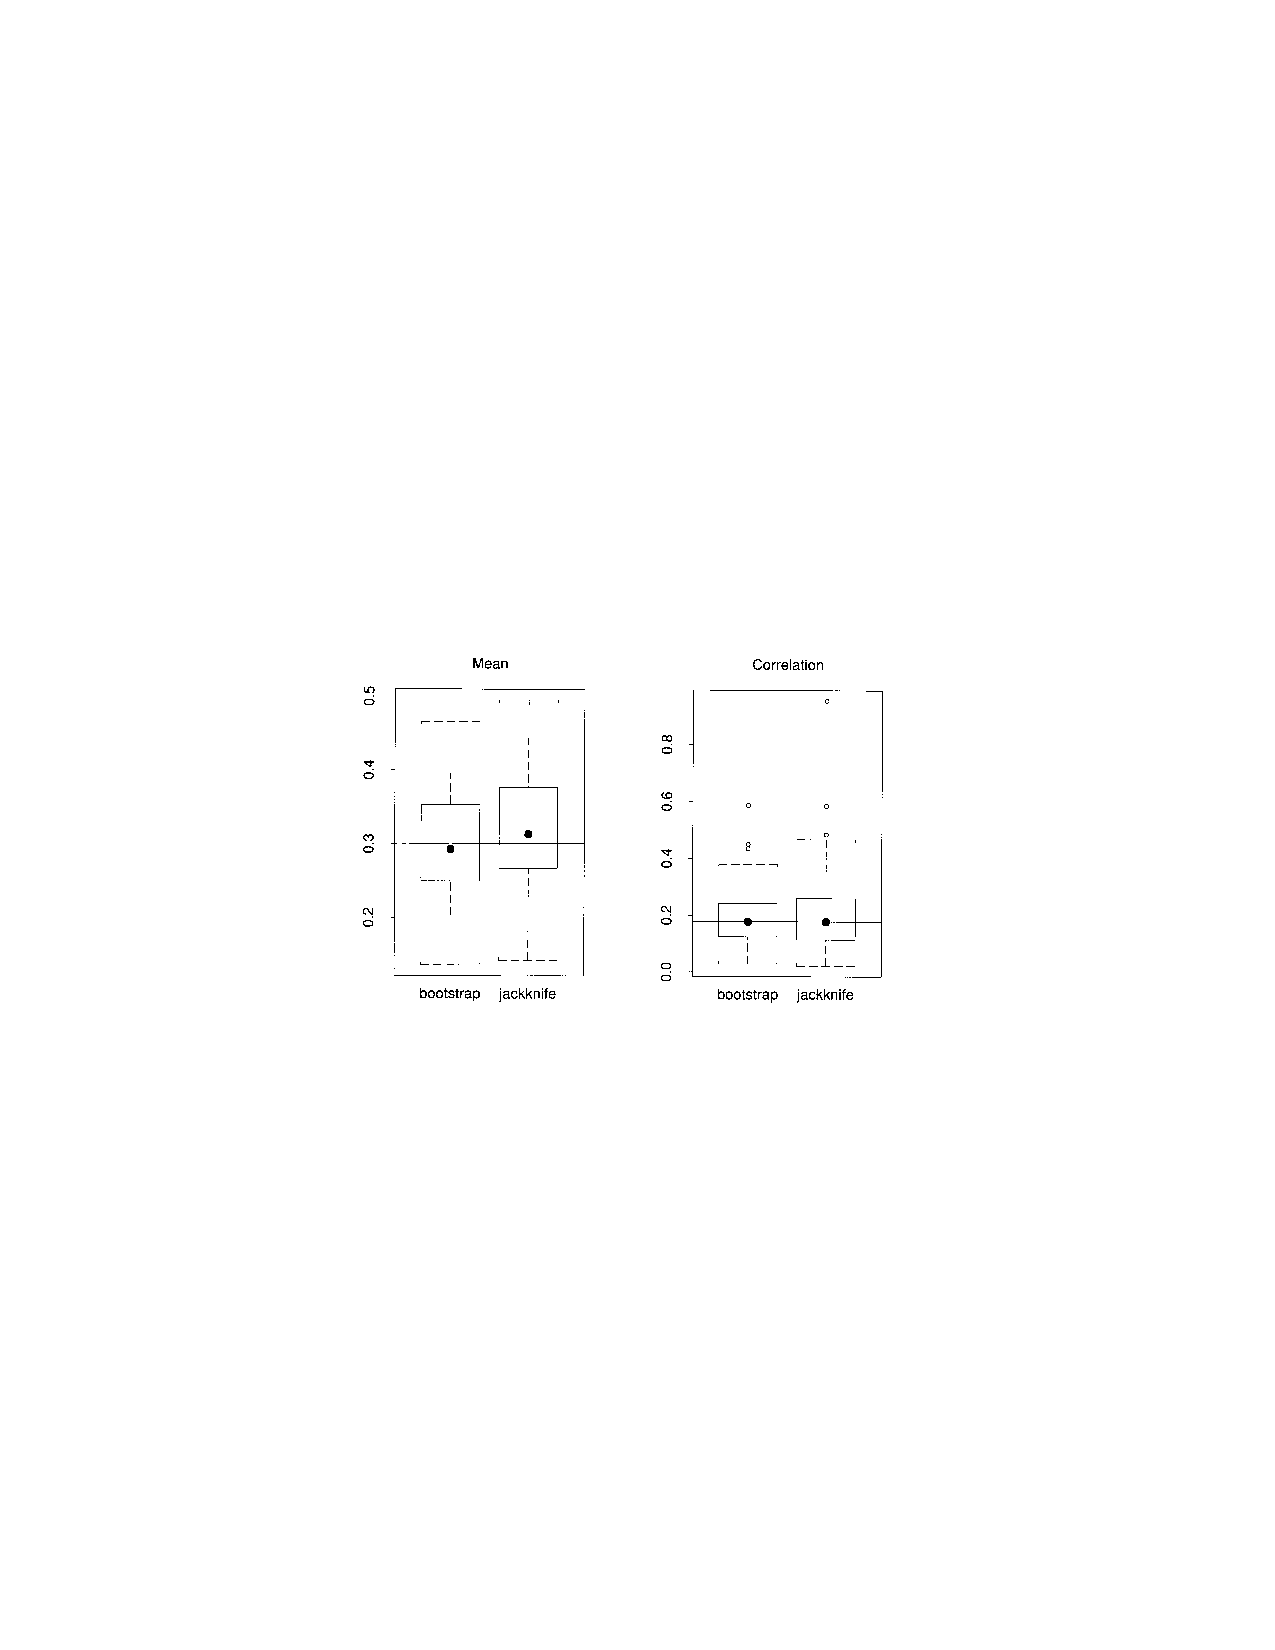
\includegraphics[height=2in]{jack-vs-boot}
\end{center}

\begin{itemize}
    \item Jackknife can be viewed as approximation to bootstrap
    \item Jackknife less computationally intensive to calculate
    \item Jackknife can fail if the statistic of interest is not `smooth' (small changes in data cause only small changes in the statistic) 
\end{itemize}    

\end{frame}

%===========================================================
\begin{frame}
  \frametitle{Loess Regression}
  
\begin{itemize}
    \item A type of non-parametric regression
    \item Basic idea -- fit a curve (or surface) to a set of data by fitting a large number of \emph{local regressions}.
    \item Cleveland, W.S. (1979). ``Robust Locally Weighted Regression and Smoothing Scatterplots". Journal of the American Statistical Association 74 (368): 829-836. doi:10.2307/2286407.
\end{itemize}

\begin{center}
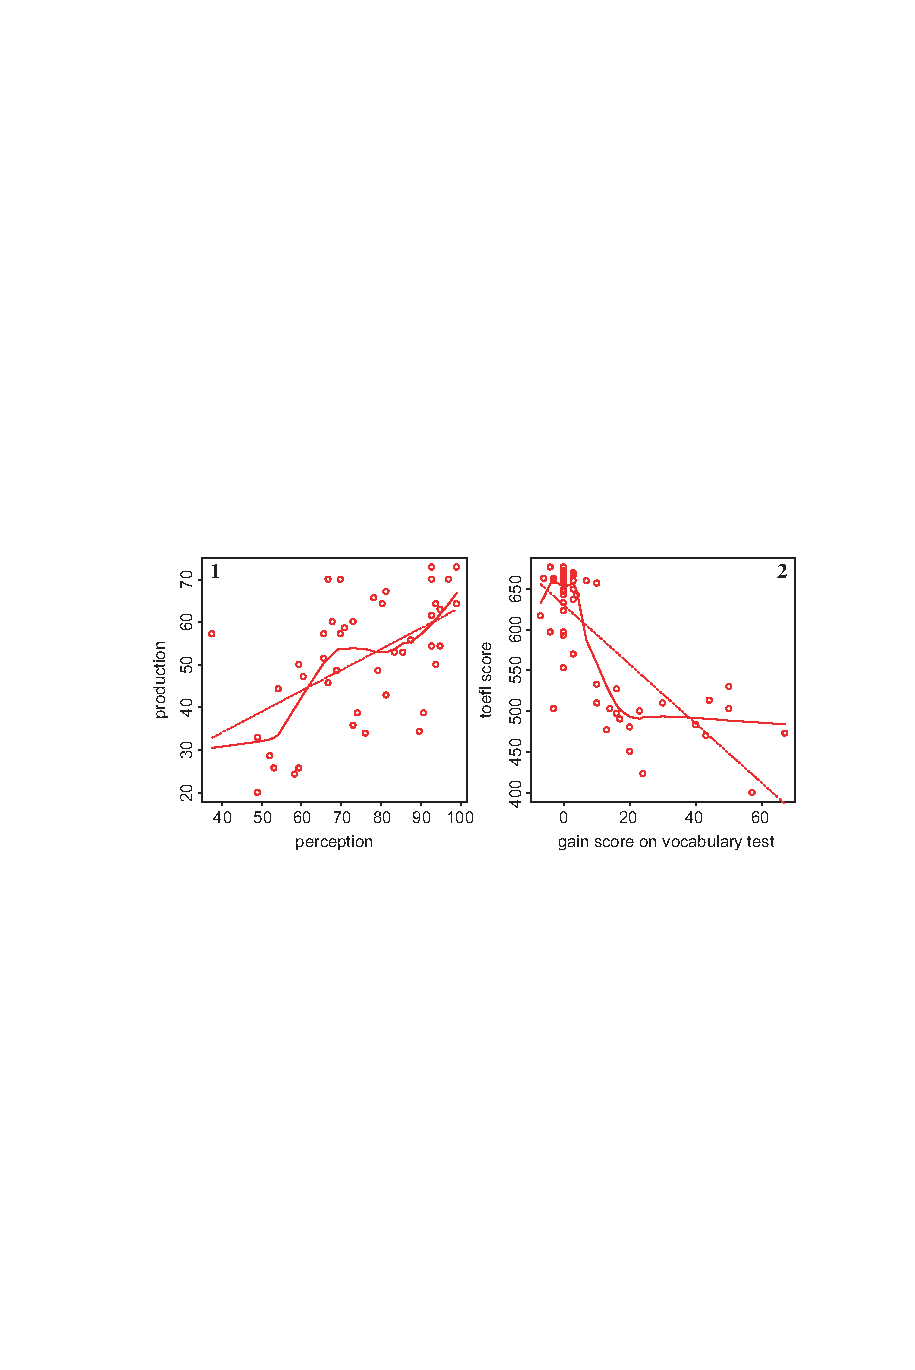
\includegraphics[height=1.25in]{loess-example.pdf}
\end{center}  


\end{frame}

%===========================================================
\begin{frame}
  \frametitle{Graphical overview of Loess fitting, I}  

{\tiny from Cleveland (1993)}
\begin{center}
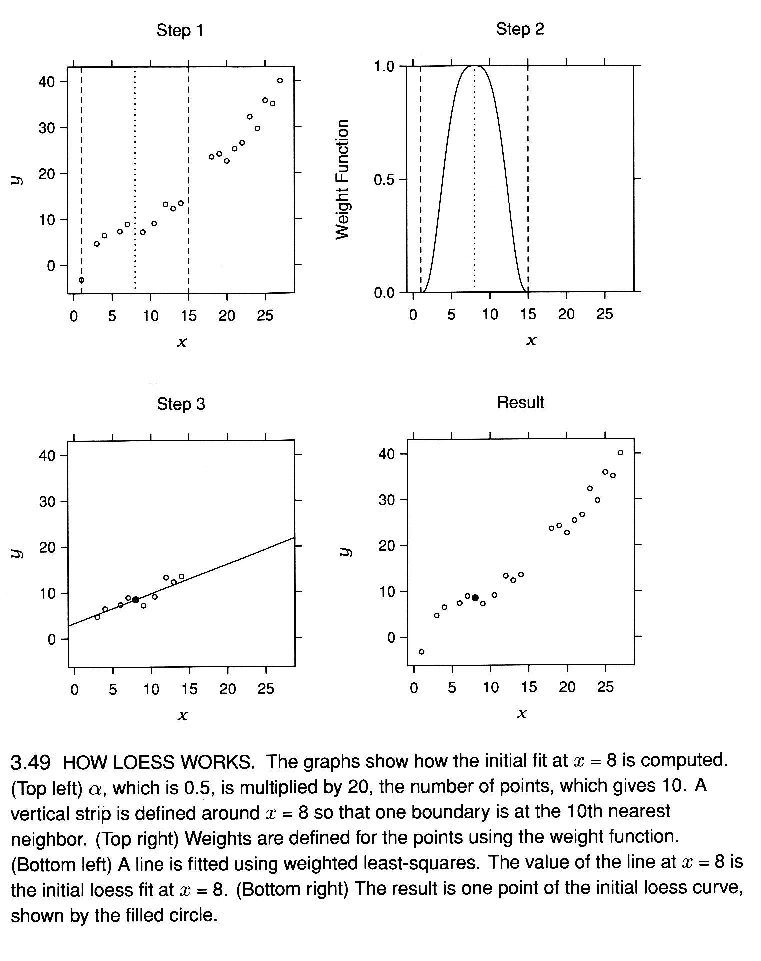
\includegraphics[height=3in]{loess1.pdf}
\end{center}  

\end{frame}

%===========================================================
\begin{frame}
  \frametitle{Graphical overview of Loess fitting, II}  

{\tiny from Cleveland (1993)}
\begin{center}
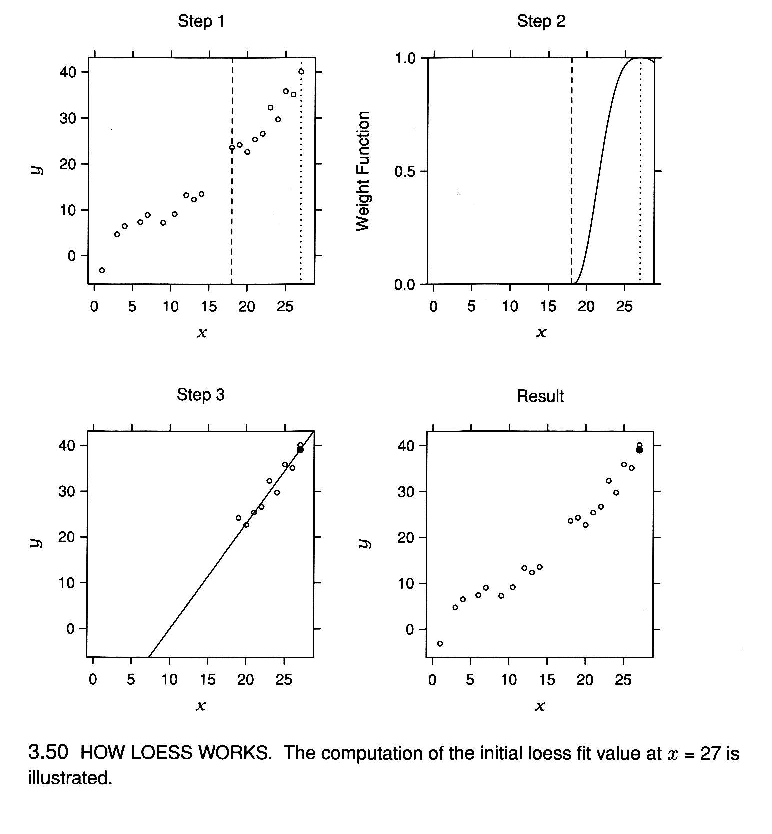
\includegraphics[height=3in]{loess2.pdf}
\end{center}  

\end{frame}

%===========================================================
\begin{frame}
  \frametitle{Graphical overview of Loess fitting, III}  

{\tiny from Cleveland (1993)}
\begin{center}
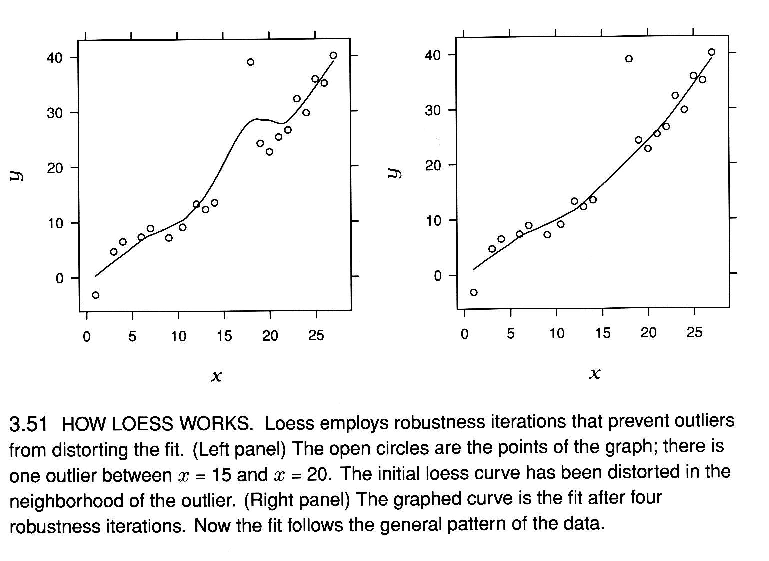
\includegraphics[height=3in]{loess3.pdf}
\end{center}  

\end{frame}


\end{document}
